%For arxiv submission
\documentclass[useAMS, usenatbib]{mnras}
\usepackage{graphicx,amsmath,color,amssymb}
%\voffset=-0.8in
%MNRAS
%\documentclass[useAMS, usenatbib, usegraphicx, twocolumn]{mnras}

\usepackage[pdftitle={A hybrid particle-analytic method for non-linear neutrino structure}]{hyperref}
% \newcommand{\eprint}[1]{\href{http://arxiv.org/abs/#1}{#1}}
% \newcommand{\adsurl}[1]{\href{#1}{ADS}}

\topmargin -1.5cm
\bibliographystyle{mnras}

\newcommand{\beq}{\begin{equation}}
\newcommand{\eeq}{\end{equation}}
\newcommand{\barr}{\begin{eqnarray}}
\newcommand{\earr}{\end{eqnarray}}

\newcommand{\rme}{\textrm{e}}
\newcommand{\rmH}{\textrm{H}}
\newcommand{\Ly}{\textrm{Ly}}
\newcommand{\pabn}{p_{\textrm{ab}}^n}
\newcommand{\pscn}{p_{\textrm{sc}}^n}
\newcommand{\rmd}{\textrm{d}}
\newcommand{\N}{\mathcal{N}}
\newcommand{\nuc}{\nu_{\rm c}}
\newcommand{\Tm}{T_{\rm m}}
\newcommand{\Tr}{T_{\rm r}}
\newcommand{\nh}{n_{\rm H}}
\newcommand{\bfA}{\boldsymbol{A}}
\newcommand{\bfr}{\boldsymbol{r}}
\newcommand{\bfV}{\boldsymbol{V}}
\newcommand{\bs}{\mathbf}
\newcommand{\mH}{\mathcal{H}}

\newcommand{\natu}{Nature (London)}
\newcommand{\aas}{Bull. Am. Astron. Soc.}
\newcommand{\gadget}{{\small GADGET\,}}

\newcommand{\spb}[1]{{\textsc{\textcolor{red}{[{\bf SPB}: #1]}}}}
\newcommand{\yah}[1]{{\textcolor{blue}{[{\bf YAH}: #1]}}}



\newcommand{\Mpch}{\,\mathrm{Mpc} \,h^{-1}}
\newcommand{\hMpc}{h^{-1}\,\mathrm{Mpc}}
\newcommand{\Lya}{Lyman-$\alpha\;$}
%%%%%%%%%%%%%%%%%%%%%%%%%%%%%%%%%%%%%%%%%%%%%%%%%%%%%%%%%%%%%%%%%%%%%%%%%%%%%%%%%%%%%%%%%%%%%%%%%%


\title{A Hybrid Particle-Analytic Method for Non-Linear Neutrino Structure}
\author[ S. Bird and Y. Ali-Ha\"{\i}moud]{
  Simeon Bird\thanks{E-mail: spb@ias.edu} and Yacine Ali-Ha\"{\i}moud\thanks{E-mail: yacine@ias.edu}\vspace{1.5mm}\\
No longer at Institute for Advanced Study, Einstein Drive, Princeton, New Jersey 08540}

\begin{document}

\date{\today}

\pagerange{\pageref{firstpage}--\pageref{lastpage}} \pubyear{2012}
\pagenumbering{arabic}
\label{firstpage}

\maketitle

\begin{abstract}
\end{abstract}

\begin{keywords}
        neutrinos - cosmology: large-scale structure of Universe - cosmology: dark matter
\end{keywords}

\section{Introduction}

Our paper is the greatest paper in the world. Blah de blah.
This paper is organised as follows. In Section \ref{sec:methods},
we describe our simulations methods. We describe our
results and compare them against other methods
in Section \ref{sec:results}. We conclude in Section \ref{sec:conclusion}.
Appendix \ref{sec:manual} is a users manual for our neutrino module.
\cite{AHB}

\section{Methods}
\label{sec:methods}

\subsection{Analytic Neutrinos}
\label{sec:analytic}

\begin{figure}
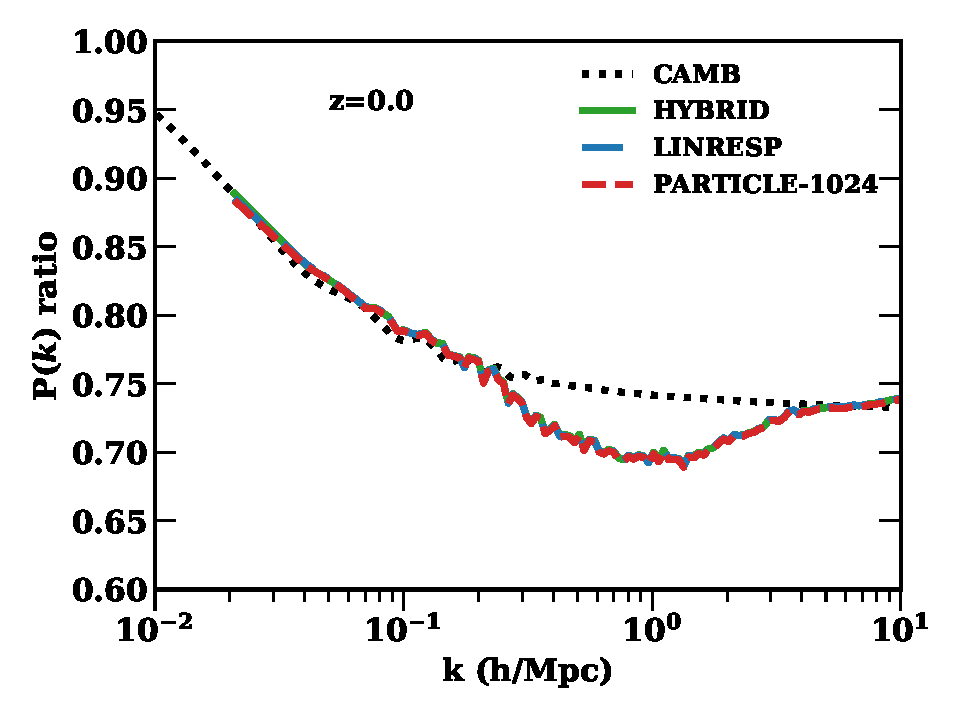
\includegraphics[width=0.45\textwidth]{nuplots/pks_rel-10.pdf}
\caption{Plot showing the matter power spectrum ratio at $z=0$ between massless neutrinos and minimal neutrino mass; one massive neutrino with a mass of $0.06$ eV.
}
  \label{fig:minimal_mass}
\end{figure}

Describe briefly the analytic particle method from the last paper.
Explain that it is extremely accurate for the pure dark matter distribution - to less than a percent.

\subsection{Particle Neutrinos}
\label{sec:particle}

Describe briefly particle method. Note that for best accuracy we are using the neutrino tree here,
and that we rebuild it every timestep to avoid the high neutrino velocities causing numerical problems.

\subsection{Hybrid Neutrinos}
\label{sec:hybrid}

Describe the method for implementing hybrid neutrinos:
particles that start as tracers, un-clustered. They sample
the Fermi-Dirac distribution with all velocities below some
initial slow value. Initially the analytic code follow the full evolution,
but then at some redshift the neutrino particles start to gravitate.

After the neutrino particles start to gravitate we modify the
analytic module so that neutrino perturbations are included only above a
minimum momentum corresponding to the initial slow value sampled by the
particle velocity distribution. In other words (insert YAH analytics here).

We use the following asymptotic expansion for the integral:
\begin{align}
 \int^\infty_{q_\mathrm{c}} \frac{j_0(qX) q^2}{e^q + 1} q^2 dq &= - \Sigma^{\infty}_{n=1} (-1)^n \frac{\exp^{-n q_\mathrm{c}}}{(n^2+X^2)^2} I_n(q_\mathrm{c},X) \;,\\
 I_n(q_\mathrm{c},X) &= (n^2 + n^3 q_\mathrm{c} + n q_\mathrm{c} X^2 - X^2) \frac{\sin(q_\mathrm{c} X)}{X} \\
 &+ (2n + n^2 q_\mathrm{c} + q_\mathrm{c} X^2) \cos(q_\mathrm{c} X)\;,\\
\end{align}
which we have confirmed, using mathematica, to be accurate to $0.1\%$.


We attempted to include neutrinos dynamically at a late time, but
accurately modelling the non-linear distortions to the analytic
Fermi-Dirac function proved overly complex. As the extra particles
do not gravitate initially, their addition at early times does
not significantly alter the efficiency of the code.


\subsection{Code improvements}
\label{sec:code}

We have altered our neutrino integrator to be a stand-alone module, largely
independent of the underlying N-body code. It should thus be easy to include
into codes other than Gadget. We have also provided a script to integrate into the
public version of Gadget-2, as well as the highly scalable public MP-Gadget
used for the BlueTides simulation. Our code is publically downloadable from.
We have added comprehensive unit tests and documentation.

\subsection{Simulations}
\label{sec:simulations}

All our simulations were run with MP-Gadget, using the scripts available
and the initial condition generator S-GenIC.

Simulations:
%TABLE OF SIMULATIONS.
\begin{table}
\begin{center}
\begin{tabular}{|l|c|c|c|l|}
\hline
% Name & $M_\nu$ (eV) & Method & Box (Mpc/h) & $N_\mathrm{part}^{1/3}$ & Notes \\
% \hline
%     &       0             &    -          & 512         & 512       &       \\
%     &       0             &    -          & 300         & 512       &       \\
%     &     0.4             &   Analytic    & 300         & 512       &       \\
%     &     0.4             &   Particle    & 300         & 512       &       \\
%     &     0.4             &   Hybrid      & 300         & 512       &  $256^3$ nu particles    \\
%     &     0.4             &   Hybrid      & 300         & 512       &  $256^3$ nu particles    \\
%     &     0.4             &   Hybrid      & 300         & 512       &  $256^3$ nu particles    \\
%     &     0.4             &   Hybrid      & 300         & 512       &  $256^3$ nu particles    \\
%     &     0.4             &   Hybrid      & 300         & 512       &  $256^3$ nu particles    \\
    Name & $M_\nu$ (eV) & Method & $N_\mathrm{nu}^{1/3}$ & Notes \\
\hline
    &       0             &    -          & 0         &    \\
    &     0.06            &   Analytic    & 0         &  Full hierarchy  \\
    &     0.4             &   Analytic    & 0         &    \\
    &     0.4             &   Particle    & 512       &    \\
    &     0.4             &   Hybrid      & 512       &    \\
    &     0.4             &   Hybrid      & 256       &    \\
    &     0.4             &   Hybrid      & 512       &    \\
    &     0.4             &   Hybrid      & 512       &  $v_\mathrm{crit}=300$  \\
    &     0.4             &   Hybrid      & 512       &  $v_\mathrm{crit}=5000$  \\
    &     0.4             &   Hybrid      & 512       &  $z_\nu = 2$  \\
\hline
\end{tabular}
\end{center}
\caption{Table of simulation parameters. All simulations have a box of $300$ Mpc/h
and $512^3$ cold dark matter particles.
}
\label{tab:simulations}
\end{table}

% Mnu = 0  (300)

% Mnu = 0.4: analytic, particle, hybrid. (300)
%
% Checks (all Mnu=0.4, hybrid, (300)):
% Varying vcrit from 500 to 300
% Varying NuPartTime from 0.333 to 0.5
% Number of hybrid particles from 256 to 512.
% Mnu = 0.06: analytic (300, 512)

%Todo:
%(300,512,1024 *neutrinos* for hybrid?)

\section{Results}
\label{sec:results}

\begin{figure}
  \caption{Projected density plot of CDM (just one plot) and neutrinos from hybrid (split into fast and slow) vs particle simulation (with shot noise)}
  \label{fig:density_plot}
\end{figure}

\begin{figure*}
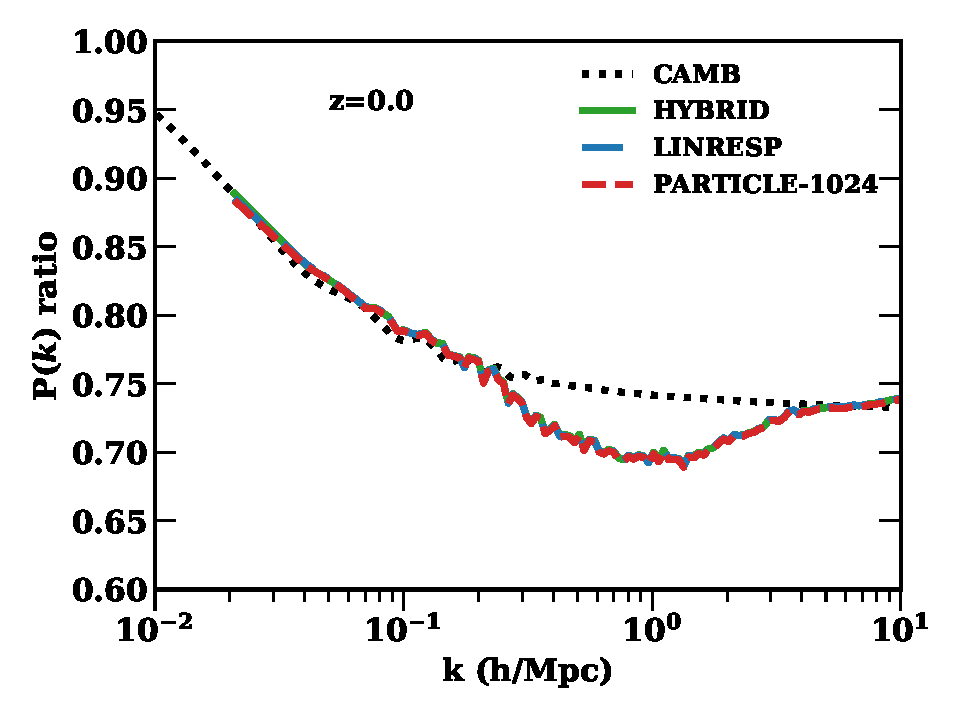
\includegraphics[width=0.45\textwidth]{nuplots/pks_rel-10.pdf}
\includegraphics[width=0.45\textwidth]{nuplots/pks_rel-0_83330.pdf}
  \caption{Plot showing the matter power spectrum ratios between analytic, particle and hybrid methods at (Left) $z=0$ and (Right) $z=0.2$. Note the slightly reduced power in the particle method - this is a consequence of the inability to correctly treat the time-varying mass of neutrinos.
  }
  \label{fig:matter_power}
\end{figure*}

\begin{figure*}
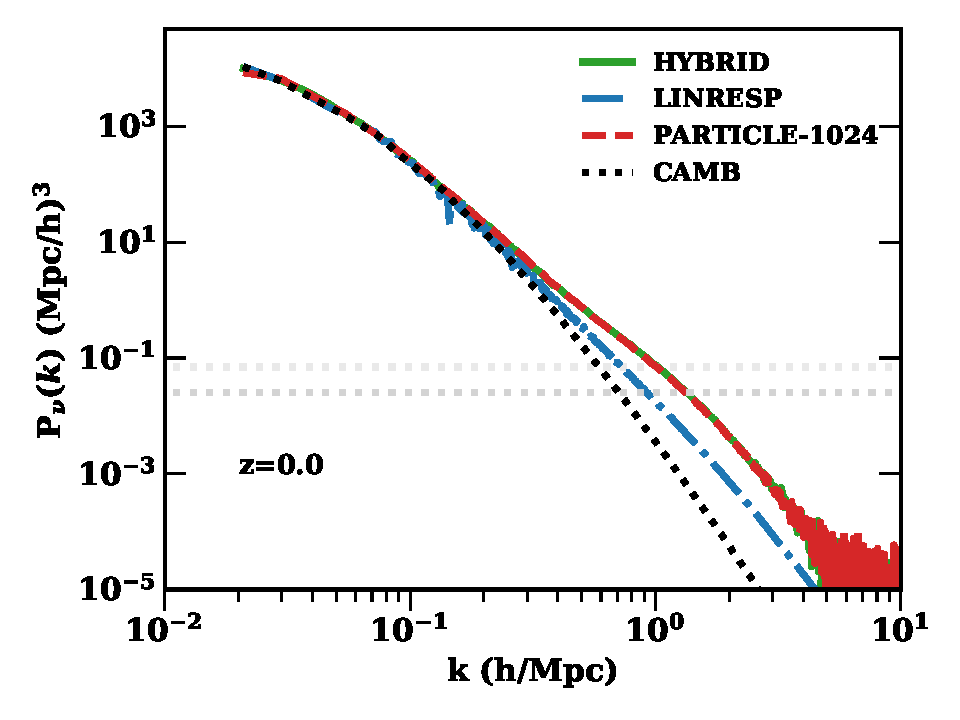
\includegraphics[width=0.45\textwidth]{nuplots/pks-nu-1.pdf}
\includegraphics[width=0.45\textwidth]{nuplots/pks-nu-0_8333.pdf}
  \caption{Plot showing the neutrino power spectrum ratios between particle, analytic and hybrid.
  (Left) At $z=0$. (Right) At $z=0.2$.
  MONEY PLOT.}
  \label{fig:neutrino_power}
\end{figure*}

There is good agreement between all methods for the total matter power.
The particle method has a slightly reduced power, which is due to our inability to
treat variable neutrino mass in the particle method.

\subsection{Numerical Checks}

\begin{figure*}
  \includegraphics[width=0.45\textwidth]{nuplots/pks-cknu-1.pdf}
  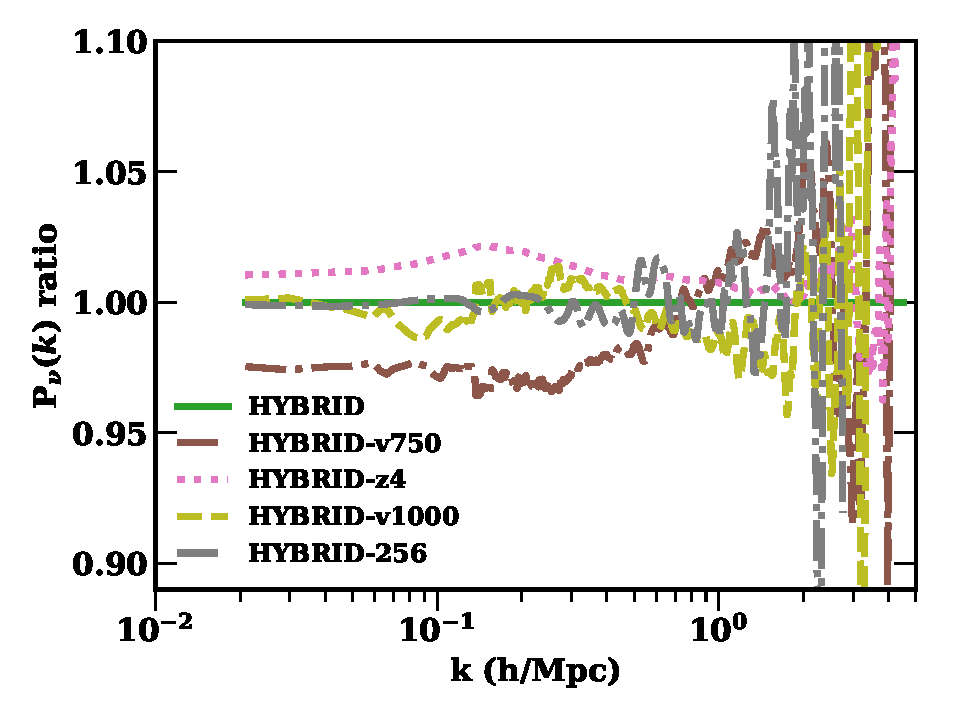
\includegraphics[width=0.45\textwidth]{nuplots/pks_nu_ckrel-1.pdf}
  \caption{Plot showing the difference in the neutrino power spectrum from changing NuPartTime and vcrit is small. Also shown is changing the neutrino particle number. We have subtracted the neutrino shot noise.}
  \label{fig:vcrit}
\end{figure*}

\begin{figure}
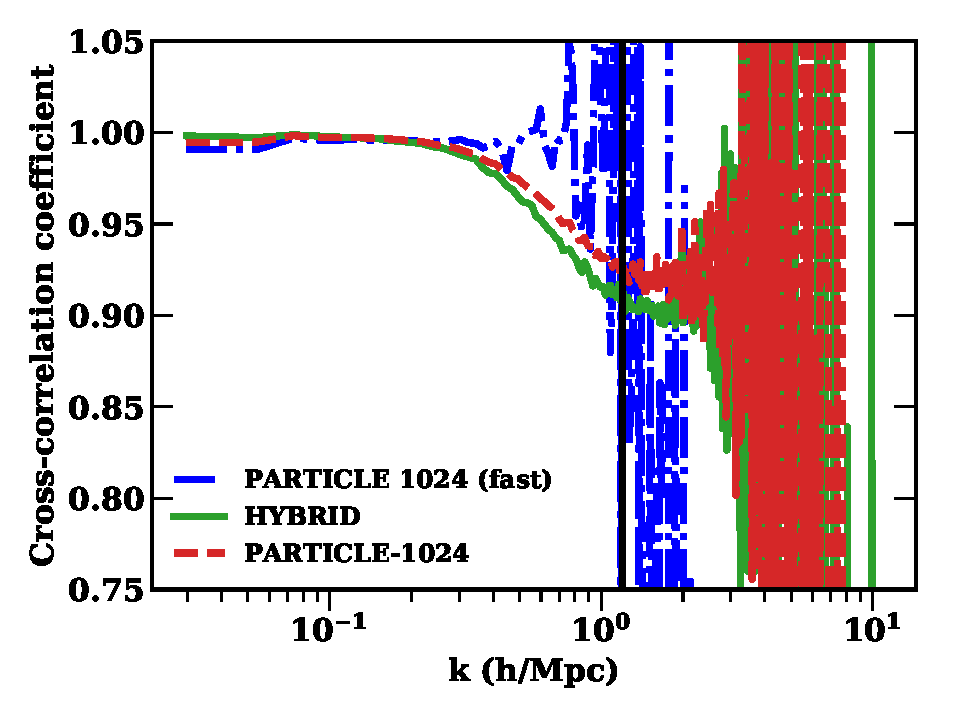
\includegraphics[width=0.45\textwidth]{nuplots/corr_coeff-1.pdf}
  \caption{Plot showing the cross-correlation coefficient between neutrinos
  and DM in particle and hybrid code, checking approximation made in analytic method.
  The cross-correlation is unity for scales where the neutrino power is not dominated by shot noise.
  \spb{Add vertical line marking this scale}
  }
  \label{fig:cross-corr}
\end{figure}


\begin{figure}
    \includegraphics[width=0.45\textwidth]{nuplots/P_nu_M500_z0.pdf}
    \caption{Plot showing CDM simulation with test particle neutrinos with fixed (not FD) single velocity of $500$ km/s at $z=0$. Neutrino power spectrum, compared to analytic $P_{CDM}$.\spb{I can't find the analytic estimates anymore...need to reproduce them}}
  \label{fig:testpart}
\end{figure}

We have checked that our results are insensitive to the time at which the hybrid neutrinos switch on,
as well as small variations in the fraction of neutrinos followed by particles or analytically. We further show that as long as we are on scales sufficiently large to avoid shot noise, our simulations are converged with respect to neutrino particle number.

Figure \ref{fig:cross-corr} shows the cross-correlation between (particle) neutrinos and CDM particles. Our analytic method implicitly assumes that this cross-correlation is unity. Figure \ref{fig:cross-corr} verifies this assumption for scales where the particle neutrino power is not dominated by shot noise. \spb{or which are larger than the neutrino free-streaming length?}

\section{Conclusions}
\label{sec:conclusion}

This problem is comprehensively solved.

Comparison with Neal's method:
computationally efficient and easy to implement.
Hybrid allows some naturally large dynamic range of N-body simulations while little shot noise.

Future work with voids, neutrino bispectrum.

\section*{Acknowledgements}

\appendix

\section{Kspace Neutrino Manual}
\label{sec:manual}

Here describe the parameters of the kspace neutrinos,
as well as the installation procedure for Gadget 2.

\section{Initial Conditions}
\label{sec:initcond}

\begin{figure*}
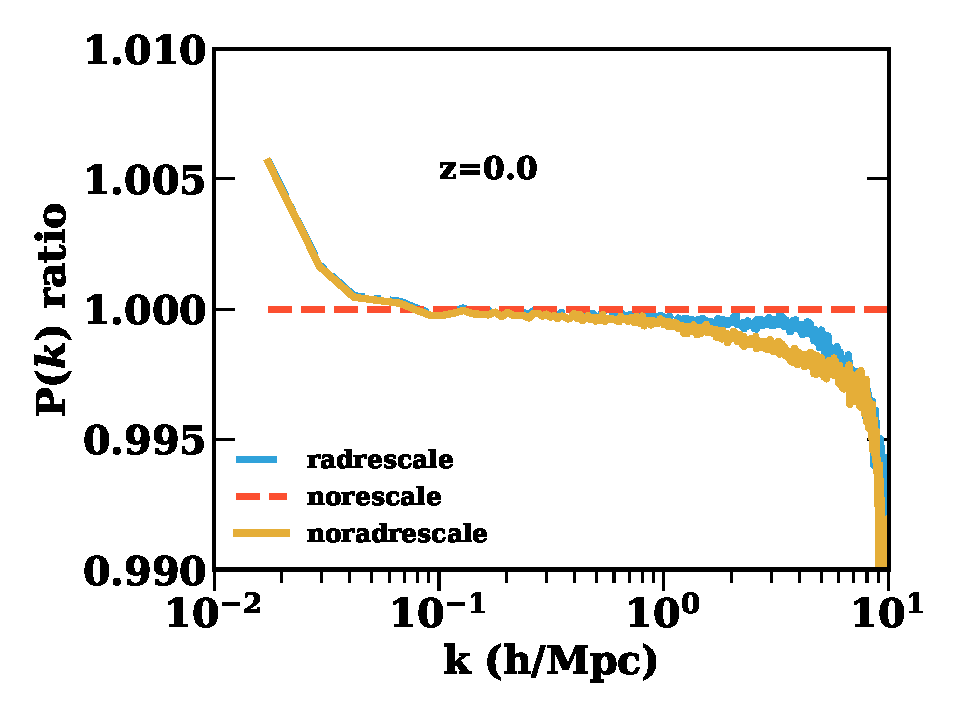
\includegraphics[width=0.45\textwidth]{icplots/pks_rel-1.pdf}
\includegraphics[width=0.45\textwidth]{icplots/pks_camb-1.pdf}
  \caption{(Left) The $z=0$ power spectrum from three simulations.
  These are initialised respectively with the $z=99$ transfer function,
  the scaled $z=0$ transfer function, and the $z=0$ transfer function
  scaled and evolved neglecting radiation density.
  Curves are normalised to the simulation using the scaled $z=0$ transfer function.
  (Right) The same three simulations normalised to the linear matter
  power spectrum from CAMB at $z=0$.}
  \label{fig:rescaling0}
\end{figure*}

\begin{figure*}
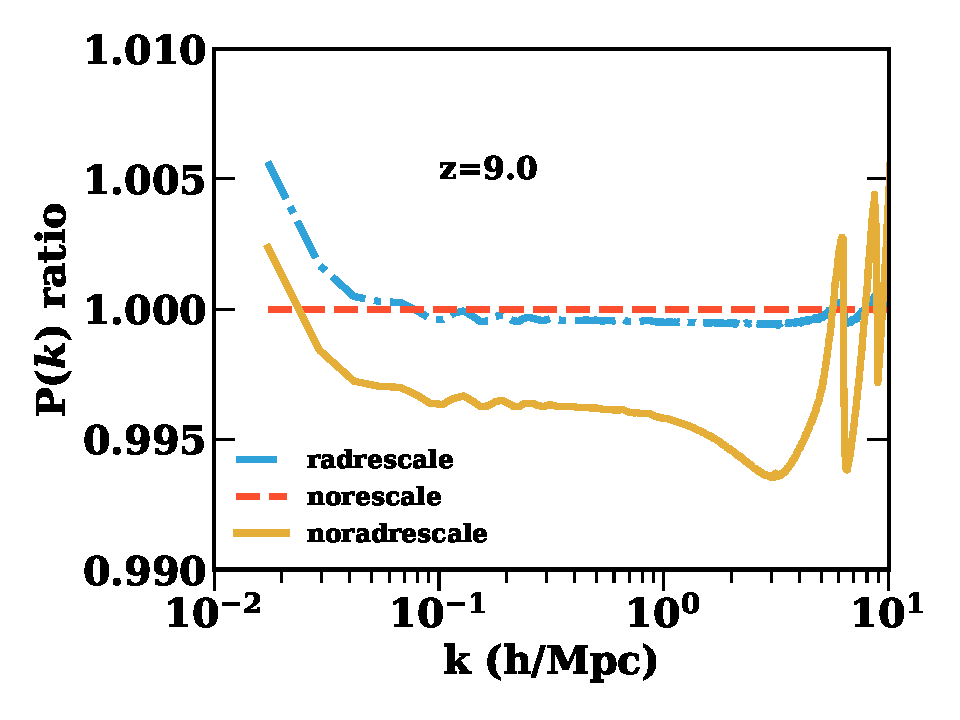
\includegraphics[width=0.45\textwidth]{icplots/pks_rel-0_1.pdf}
\includegraphics[width=0.45\textwidth]{icplots/pks_camb-0_1.pdf}
  \caption{(Left) The $z=10$ power spectrum from three simulations.
  These are initialised respectively with the $z=99$ transfer function,
  the scaled $z=0$ transfer function, and the $z=0$ transfer function
  scaled and evolved neglecting radiation density.
  Curves are normalised to the simulation using the scaled $z=0$ transfer function.
  (Right) The same three simulations normalised to the linear matter
  power spectrum from CAMB at $z=0$.}
  \label{fig:rescaling10}
\end{figure*}

%Show higher redshift?

Since \cite{AHB}, we have improved our initial conditions, generated
using our freely available initial conditions code
S-GenIC \url{https://github.com/sbird/S-GenIC}. These improvements concern
the relationship between velocities and displacements in Lagrangian perturbation theory.
\citep{Zeldovich_1970, Scoccimarro_1998}. In linear Lagrangian perturbation theory,
velocities and displacements are related by a scale-independent factor

\begin{equation}
v(k) = a H(a) \frac{d \log D(a)}{d \log a} \delta(k)
\label{eq:vel_prefac}
\end{equation}
where $D(a)$ is the linear growth function and $H = \dot{a}/a$, the Hubble function.
In \cite{AHB}, the Hubble function used in Eq.~\ref{eq:vel_prefac}
neglected radiation density, leading to a small error.

Furthermore, in matter domination, the derivative of the linear growth function,
$\frac{d \log D(a)}{d \log a}$, was approximated by \citep{Bouchet:1995}
\begin{equation}
\frac{d \log D(a)}{d \log a} \approx \left(\frac{\Omega_M a^{-3}}{\Omega_M  a^{-3} + \Omega_L}\right)^{0.6}\,.
\end{equation}
However, this approximation neglects the radiation density, which becomes
non-negligible at $z > 50$. This is important particularly when considering
massive neutrinos, because at high redshift neutrinos are slightly relativistic,
and thus the background density depends slightly on the neutrino mass.

In practice these two approximations partially cancelled, leading
to results that were correct to a couple of percent. However, we
have now removed them both and use both the full Hubble function
and obtain $\frac{d \log D(a)}{d \log a}$ by numerically solving
the linear growth equation \citep{Peebles:1993}:
\begin{equation}
\frac{d}{da}\left(a^3 H(a) \frac{d D(a)}{da}\right) - \frac{3}{2} \frac{a \Omega_M}{H(a)} D(a) = 0
\end{equation}
subject to initial conditions at $z \gg 100$ corresponding
to the exact growing mode in a matter-radiation universe \citep{Groth:1975}
\begin{equation}
  D(a_i) = \Omega_r + \frac{3}{2} \Omega_M a_i\,.
\end{equation}

In the presence of baryon or neutrino fluids, the scale-independence
of the growth function is itself an approximation. For neutrinos, this
is because the free-streaming scale is redshift dependent. For baryons
it is because the baryons initially couple to the photons, suppressing
their power on scales which are sub-horizon at $z \sim 1100$. However,
by $z=99$ the baryons have already fallen into
the potential wells generated by the CDM,
and $\delta_\mathrm{b} \approx 0.7 \delta_\mathrm{CDM}$.
\cite{Zennaro_2017} showed this effect to induce only
a sub-percent error for our scales of interest and hence we neglect it.

We choose to generate our initial conditions using the CAMB total matter transfer
function at $z=99$. An alternative is to generate initial conditions
using the $z=0$ transfer function, scaled by $D(99)/D(0)$. This can
be used to account for background radiation density, if radiation is not included
in the background evolution. Even if radiation is included, it can account
for radiation perturbations and other relativistic effects on the scale
of the horizon at $z=99$ \citep{Zennaro_2017}. It also naturally accounts
for the fact that our single fluid simulations are unable to accunt for
the different growth rates experienced by baryons and CDM.

In Figure \ref{fig:rescaling0} we show the differences between the $z=0$
power spectra produced using the $z=99$ transfer function, the
scaled $z=0$ transfer function, and the $z=0$ transfer function
scaled and evolved neglecting radiation density.
For our scales of interest, these differences are slight,
especially compared to the variance induced by our finite box size.
Thus we use the $z=99$ transfer function as it is practically and conceptually simple,
whereas the linear scaling becomes complex in the presence of massive neutrinos.

Note the differences on small scales between the simulations which
include radiation in the background and the simulations which do not.
This is due to the linear growth being underestimated
at $z > 10$ in the simulations without radiation. On scales which are
already non-linear at these redshifts, non-linear growth will be inaccurately
computed. Although this effect is small, we nevertheless suggest that simulations
which use scaled $z=0$ transfer functions still include radiation in the background.
Note also that simulations with boxes $\gtrsim 2$ Gpc should somehow account
for radiation and relativistic effects.

\label{lastpage}

\bibliography{neutrinos}

\end{document}
